\chapter{Implementation}

In this section, we describe the design and technical decisions that are required to implement a decentralized photo verification system that allows photo authenticity to be verified by an application of Ethereum smart contracts with a combination of cryptographic hash and Merkle Tree structures. The system provides a tamper proof environment where photo hashes and metadata are stored securely on the blockchain in such a way that any changes could be detected.

Ethereum blockchain is used to build the application and Solidity is used for smart contract development, which stores cryptographic hashes of photos and their metadata. By using this approach, we present a way to minimize gas fees while offering scalable verification which allows any user to verify photo authenticity using accounts either on full or partial metadata. To guarantee non tamperable operations, the app utilizes iOS specific security features such as Secure Enclave and code signing.

The app stores only hashes of the images and metadata and therefore avoids unnecessary storage costs but once registered, photo authenticity cannot be modified. The following section will discuss the significant components such as: smart contract structure, Merkle tree hashing, platform choice, and UI flows.
\break
\section{Platform Choice: IOS}
The decision to build the application on iOS rather than Android was primarily influenced by iOS's closed ecosystem, strong security features, and the advanced cryptographic capabilities available on iOS devices. Apple’s platform offers a highly secure environment for mobile applications, which is crucial when dealing with photo integrity and blockchain interactions.
The iOS platform provides a range of security features, including the Secure Enclave, which is a dedicated hardware component that securely stores cryptographic keys and performs cryptographic operations. This feature is particularly beneficial for our application, as it allows us to securely manage the private keys used for signing transactions on the Ethereum blockchain.

\subsection{Rationale}

\begin{table}[bt]
    \centering
    \begin{tabularx}{\textwidth}{|X|X|X|}
    \hline
    \textbf{Security Feature}  & \textbf{Android}  & \textbf{iOS} \\ \hline
    Reverse Engineering        & Easily accessible APK files, decompiling with tools like JADX, JADX-GUI  & Difficult to reverse-engineer, code obfuscation in place, strict app store guidelines \\ \hline
    Code Signing               & APK signature required, but root access can bypass code signing & Strict code signing required, Apple’s strict app store review process \\ \hline
    Security                   & Vulnerable to malware, less secure app permissions, security patches depend on device manufacturer & More secure with app sandboxing, fewer vulnerabilities, regular security updates from Apple \\ \hline
    Developer Certificates     & Developers use a keystore to sign apps, no centralized certificate authority & Centralized certificate authority for all app distribution, stricter control over certificates \\ \hline
    \end{tabularx}
    \caption{Security Features Comparison Between Android and iOS}
    \label{tab:securityFeatures}
\end{table}

\begin{itemize}
    \item {\textbf{Closed Ecosystem:}} iOS's closed ecosystem provides a more controlled environment for app development and distribution. This reduces the risk of malware and unauthorized modifications, which is particularly important for an application that deals with sensitive data such as photo hashes and metadata. iOS’s tightly controlled ecosystem ensures that apps undergo rigorous vetting and approval processes, reducing the likelihood of malware and unauthorized modifications \cite{iosSecGarg}
    \item {\textbf{Code Signing and App review:}} A developer certificate from Apple needs to sign all iOS applications in order to prevent post-publication modifications of app code. The app's security relies on developer-signed certificates thus tampering attempts will make the application useless for malicious intent \cite{devCert}.
    \item {\textbf{Secure Enclave:}} iOS incorporates Secure Enclave as a hardware-based processor to secure operations involving cryptographic keys and authentication. The hardware-backed security function delivers specific advantages to Ethereum private key storage by guarding it from unauthorized intruders \cite{SecureEnclave2024}.
\end{itemize}




\section{Smart Contract and Blockchain Design}
The smart contract forms the core component of our decentralized photo verification system. It is the main responsible agent for storing the cryptographic hashes of photos and their associated metadata on the Ethereum blockchain. The smart contract is designed to be efficient and cost-effective, while also ensuring secure storage and retrieval of photo hashes and metadata.

The  photo verification system is built on top of the Ethereum blockchain \cite{ethereuem}, a programmable and decentralized database that allows running smart contracts self-executing code snippets that execute in a trustless environment. Ethereum's popularity stems from its mature ecosystem, decent developer support, and fully featured toolchains, which make it an ideal candidate to store immutable and verifiable digital assets.

The application uses ERC721 standards to store unique photo entries which were initially established for NFTs  \cite{erc721}. ERC20 tokens are interchangeable but ERC721 tokens serve as unique digital items because they represent one-of-a-kind digital content like hashes derived from images along with their metadata. The ERC721 standard provides unique tokenId assignment for each token which serves perfectly for blockchain identity photo associations.

ERC721 implements three essential components which include ownership policies for digital assets along with transfer protocols and automatic event recording machinery for proving asset origins. The main benefit of using ERC721 in this project is its capability to link a hash with one individual user for both immutable tracking purposes.

\begin{figure}
    \centering
    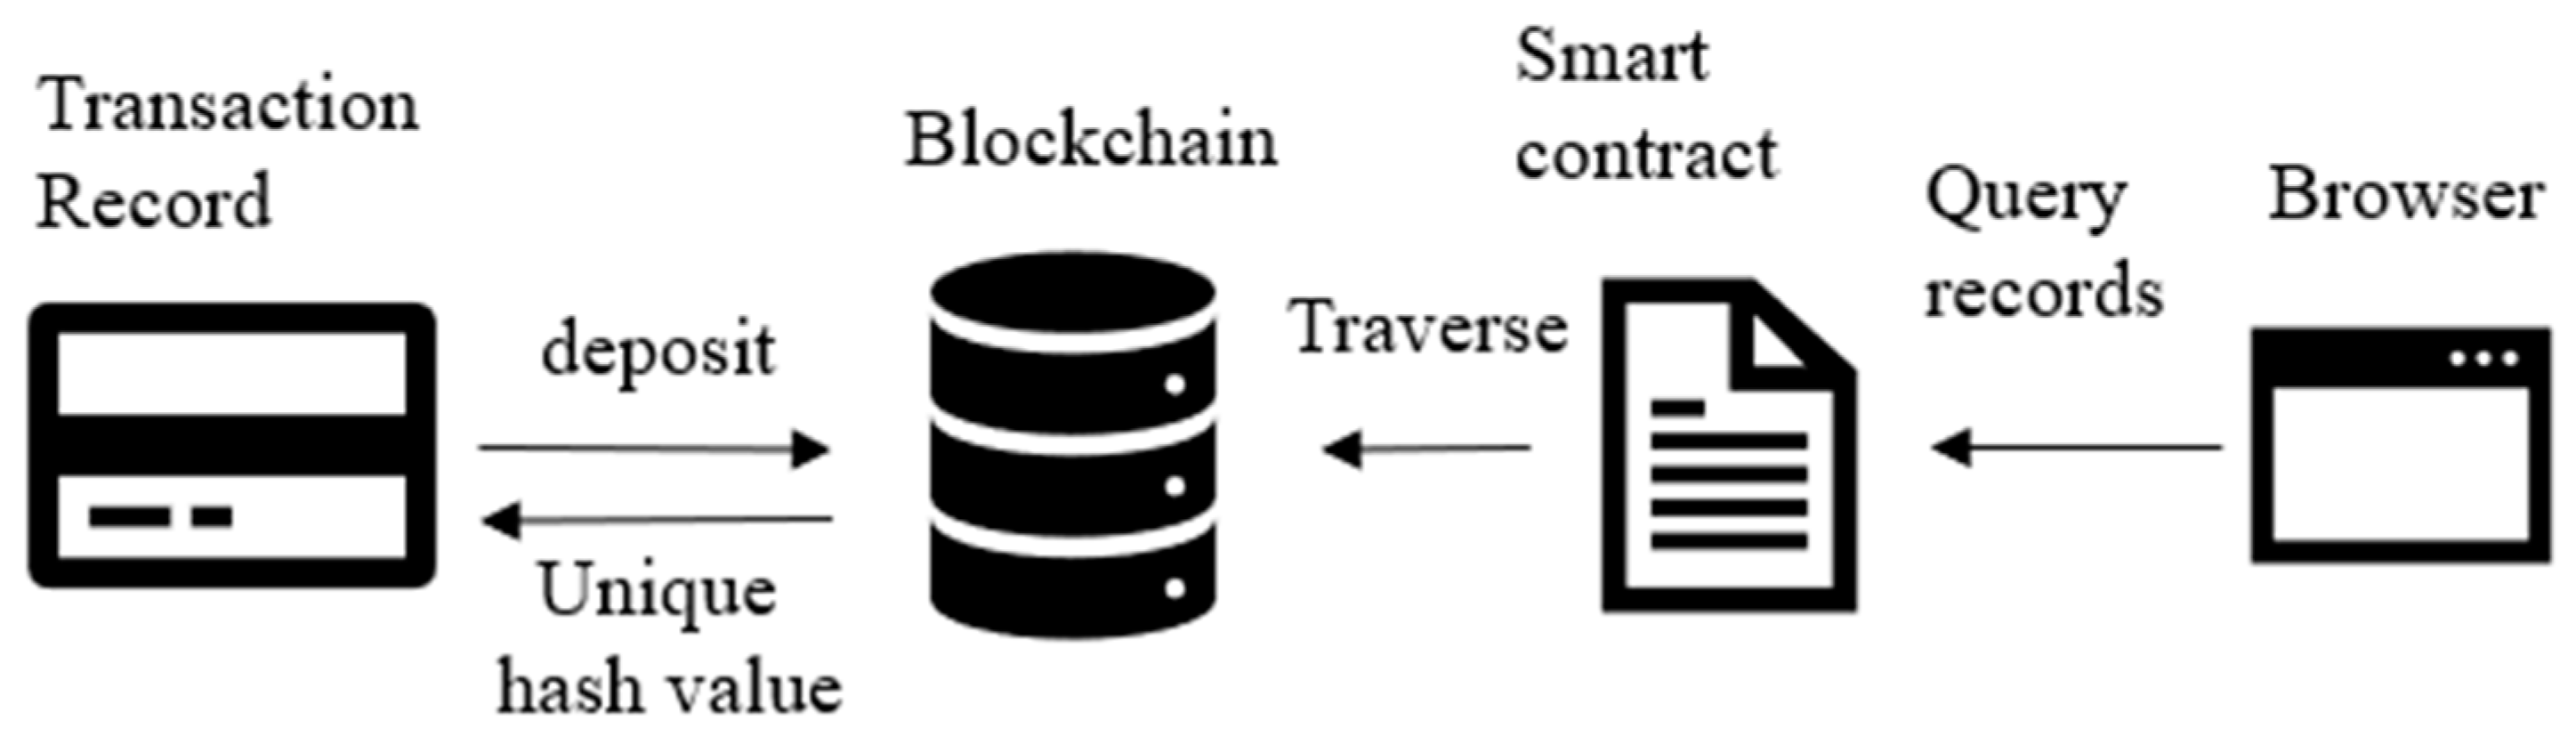
\includegraphics[scale=0.1]{images/smartContractArch.png}
    \caption{General smart contract architecture.}
    \label{fig:smartContractArch}
\end{figure}

\subsection{Tokenization and the Role of ERC721}
The ERC721 standard functions as an Ethereum protocol which provides features to track and produce non-fungible tokens (NFTs). Under this standard every token possesses a separate tokenId which serves as its distinct identification while it can be assigned to a user. The Merkle root hash which originates from photo data and metadata functions as the singular identification mark of images for this project. The proof-of-existence and ownership functions are encoded as ERC721 token while the unique fingerprint is simultaneously added to blockchain data

\noindent{The use of ERC721 allows the system to:}
\begin{itemize}
    \item Guarantee that no two photos are associated with the same token.
    \item Allow photo owners to query or retrieve ownership proof at any time.
    \item Maintain an audit trail of all registered hashes.
    \item Utilizes standard Ethereum wallets for identity linkage.
    \item Storing metadata associated with the image hash, if required in the future.
    \item Allow users to transfer ownership of the token to another address.
    \item Provide a mechanism for public verification of the hash.
\end{itemize}

This framework aligns with blockchain best practices for managing verifiable, user-bound assets in a decentralized system

\subsection{Smart Contract Overview}
The system features a Solidity smart contract that runs on the Ethereum Sepolia Testnet. The smart contract is responsible for managing the registration and verification of photos, as well as storing the associated metadata if necessary. The smart contract includes functions for:

\begin{itemize}
    \item Registering a unique image hash, derived from the Merkle tree root.
    \item Minting a non-fungible token to represent the image’s existence and ownership.
    \item Enabling public verification of hashes by checking if a hash exists and is associated with a specific address.
\end{itemize}

\textbf{Storing Hashes for Cost Efficiency: }
The main drawback of blockchain-based storage involves its high price tag. Blockchain-based storage becomes too expensive when users attempt to store large images particularly those with high-resolution photos. We maintain only cryptographic hash values of images together with their necessary metadata while ensuring both security and affordability.


\subsection{Contract Design and Structure}
The PhotoProof smart contract built with Solidity programming language extends OpenZeppelin ERC721 base implementation to build a secure system that verifies photo ownership. The smart contract establishes two fundamental mapping relationships between Merkle Root hashes (bytes32) and Ethereum wallet addresses of owners and between owners and their registered hash collections.

The mappings operate as essential components for establishing a tamper-evident system which binds photos to their original owners and enables ownership history verification.

\noindent{Below is the simplified core contract:}
\lstinputlisting[language=Solidity, caption={Core contract for the PhotoProof system}, captionpos=b]{code/photoProof.sol}

\noindent{The contract includes the following key components:}
\begin{itemize}
    \item {\textbf{\textit{photoHashToOwner} Mapping: }} A one-to-one map linking each unique photo hash (Merkle Root) to the owner's Ethereum address.
    \item {\textbf{\textit{ownerToHashes} Mapping: }} Allows any user to register a new photo hash. If the hash already exists, it is rejected to prevent duplicate claims.
    \item {\textbf{\textit{registerHash(bytes32)} Function: }} Registers a new SHA-256 hash on-chain. If the hash is already registered, it is rejected. Otherwise, a new ERC721 token is minted for the sender, and the hash is stored in both photoHashToOwner and the sender’s history. This operation emits a HashRegistered event to enable external systems to listen and audit the transaction.
    \item {\textbf{\textit{verifyHash(bytes32)} Function: }} This function allows users to verify if a specific hash is registered and associated with a particular owner. It returns a boolean value indicating the verification status.
\end{itemize}

The contract maintains a minimal structure which decreases the associated gas expenses. The approach follows optimization methods that researchers discuss in smart contract security literature \cite{blockChainAndBeyod}.

The hash data type uses bytes32 to support SHA-256 output while minimizing storage requirements. The contract avoids storing metadata or image content because storing large datasets on Ethereum proves too expensive. The system performs off-chain calculations and verifies results on-chain to maintain an economical structure that upholds integrity.


\section{Merkle Tree Hashing for Scalable Verification}
A basic cryptographic hash of an image generates a unique fingerprint yet proves inadequate for strong verification because it does not work well with incomplete metadata. The system solves this problem through Merkle Tree hashing which creates a hierarchical cryptographic data structure that verifies proofs in both their entirety and parts while maintaining high efficiency and preventing tampering.

The Merkle Tree which blockchain systems initially used for data integrity verification operates as a binary hash tree that uses leaf nodes to store hashed data items (metadata fields or image content) and non-leaf nodes to store hashes of their child nodes. The Merkle Root functions as the top node which contains the summary of all inputs. The digital authentication workflow benefits from this structure because it allows quick proof-of-inclusion checks and rapid updates and minimal recomputation when data changes \cite{forensicAnalysisOfJPEG}.

\begin{figure}
    \centering
    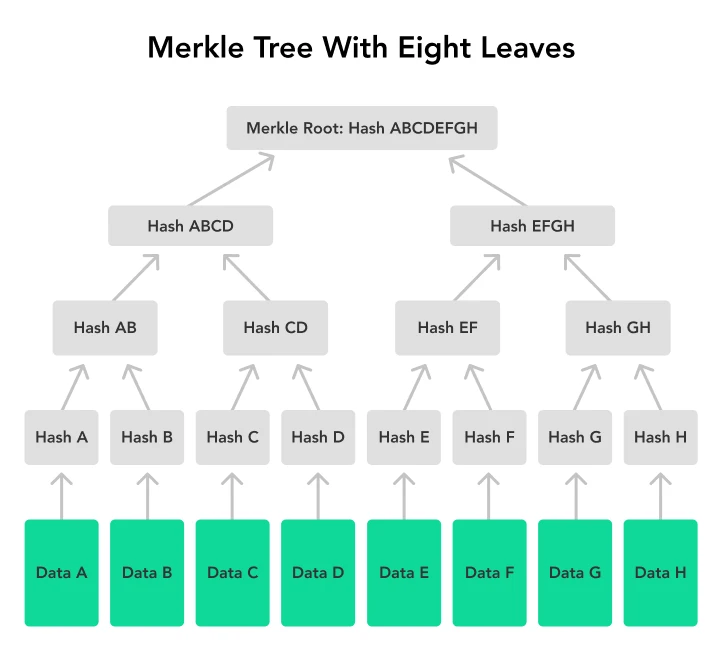
\includegraphics[scale=0.5]{images/merkleTreeHash.png}
    \caption{Merkle Tree Hashing process.}
    \label{fig:merkleTree}
\end{figure}


\subsection{Use Case in Photo Authenticity}
In the proposed system, a Merkle Tree is constructed from a combination of the following data elements:
\begin{itemize}
    \item Image content (hashed in base64 format),
    \item Device-specific EXIF metadata (e.g., make, model, resolution),
    \item Contextual data (e.g., geolocation, timestamp),
    \item App-specific attributes (e.g., app version, owner address).
\end{itemize}

The SHA-256 hashing process applies to each value separately before recursive combination produces a single root hash for image verification. The blockchain registers the Merkle Root by utilizing the smart contract described in Section 3.2.

This design enables two major capabilities:
\begin{itemize}
    \item {\textbf{Full Verification::}} When the full image and metadata are available, the complete Merkle Tree can be reconstructed to validate the photo.
    \item {\textbf{Partial Verification:}} If only select metadata fields are available (e.g., timestamp and device), the system can compute a partial Merkle path to verify that these elements match the original hash, without revealing all information.
\end{itemize}

The system operates with flexibility to protect privacy while maintaining efficiency during authentication processes that require users to verify authenticity without revealing complete image content.

\subsection{Hashing Pipeline}
The app implements the following sequence during Merkle Tree construction:
\begin{itemize}
    \item {\textbf{Image Capture:}} User takes a photo in the app.
    \item {\textbf{Metadata Extraction:}} EXIF fields are parsed from the image using iOS APIs.
    \item {\textbf{Field Hashing:}} Each metadata field and the image itself are individually hashed using SHA-256.
    \item {\textbf{Tree Formation:}} Hashes are combined recursively into a binary tree to compute the Merkle Root.
    \item {\textbf{Blockchain Storage:}} The final root hash is stored via the registerHash() function in the smart contract.
\end{itemize}

The hashing method implements robust image hashing principles described by Venkatesan \cite{robustImageHashing} in his original work while adding hierarchical trees to enhance flexibility and tamper-resistance along with compact proof functionality.

\subsection{Security and Efficiency}
Merkle Trees provide a significant advantage in environments where data integrity and selective disclosure are required. Even if only a subset of metadata is available or needs to be disclosed, the Merkle Tree enables:
\begin{itemize}
    \item {\textbf{Compact proof generation:}} Instead of resending all data, only a small set of hashes and tree paths is required.
    \item {\textbf{Tamper detection:}} Any change in image content or metadata will result in a different root hash.
    \item {\textbf{Fast verification:}} Tree operations can be executed in logarithmic time, allowing for efficient recomputation on mobile devices.
\end{itemize}
For potential future integration with zero-knowledge proofs, newer hash functions like Poseidon \cite{poseidon} could be explored, offering enhanced performance in recursive zkSNARK-compatible environments.

\section{Hashing Mechanism and Metadata Selection}
A cryptographic hash generated from image content together with critical metadata sections forms a tamper-proof identity for every photo. The Merkle Root functions as an unalterable photo fingerprint by storing the computed hash. The hashing system operates to produce new hashes when any minor change occurs in image data or metadata which indicates photo tampering.

\subsection{Metadata Selection Criteria}
Data obtained from digital photos through Exchangeable Image File Format (EXIF) reveals essential origin details along with technical specifications about digital images. The reliability and stability of EXIF fields differ between different devices and image processing workflows. A selected set of fields was established for this system through an assessment of reliability and entropy and their impact on verifiability.

\noindent{The selected fields include:}
\begin{itemize}
    \item {\textbf{Device Details:}} Used to bind the image to the specific hardware that captured it. These include:
    \begin{itemize}
        \item \textit{CameraMake}
        \item \textit{CameraModel}
        \item \textit{LensModel}
    \end{itemize}

    \item {\textbf{Time Data:}} Establishes the temporal authenticity of the image. The timestamp of when the photo was taken is crucial for establishing the context and authenticity of the image. This includes:
    \item \begin{itemize}
        \item \textit{DateTimeOriginal}
        \item \textit{DateTimeDigitized}
        \item \textit{CreationTime}
    \end{itemize}

    \item {\textbf{Location Data:}} Provides geographic context and enables geolocation verification. This includes:
    \begin{itemize}
        \item \textit{GPSLatitude}
        \item \textit{GPSLongitude}
        \item \textit{GPSAltitude}
    \end{itemize}

    \item {\textbf{Image Geometry:}} Identifies the original resolution and prevents downsampling or cropping manipulation. This includes:
    \begin{itemize}
        \item \textit{ImageWidth}
        \item \textit{ImageHeight}
        \item \textit{PixelWidth}
        \item \textit{PixelHeight}
    \end{itemize}

    \item {\textbf{Exposure and Optics:}} Adds a layer of verification tied to camera behavior. This includes:
    \begin{itemize}
        \item \textit{ApertureValue}
        \item \textit{ShutterSpeedValue}
        \item \textit{FNumber}
        \item \textit{FocalLength}
        \item \textit{ExposureTime}
        \item \textit{BrightnessValue}
    \end{itemize}

    \item {\textbf{File Metadata:}} Helps track file integrity and detect post-processing. This includes:
    \begin{itemize}
        \item \textit{AssetId}
        \item \textit{ModificationTime}
        \item \textit{ColorModel}
    \end{itemize}
\end{itemize}

\begin{figure}[ht!]
    \centering
    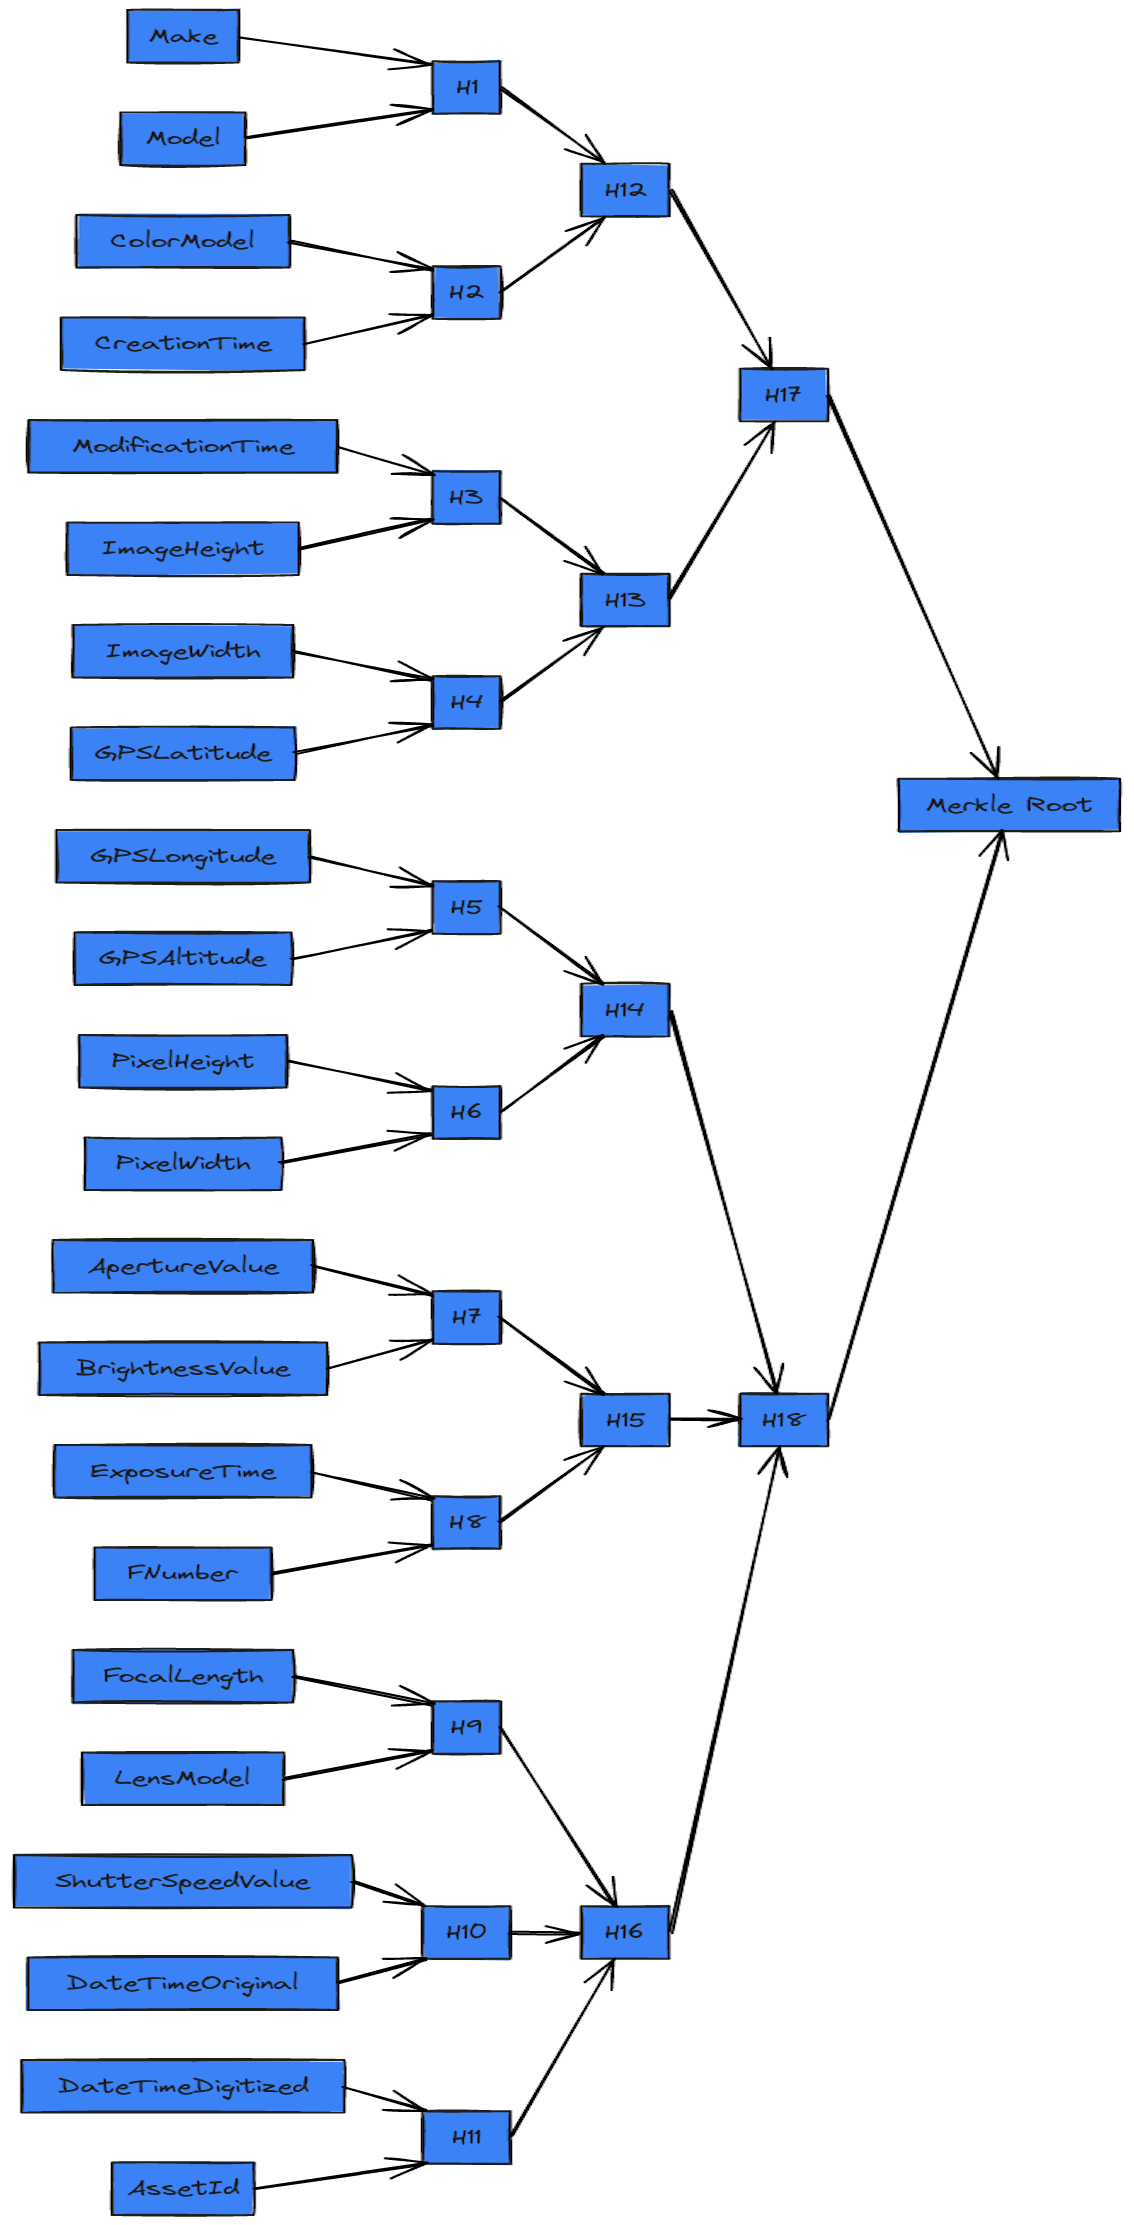
\includegraphics[scale=0.245]{./images/merkleHashComputation.png}
    \caption{Merkle Hash Computation using Exif Metadata}
\end{figure}

Each field receives individual hashing before the Merkle Tree formation enables both complete and partial verification methods (Section 3.3).
The selected metadata fields are chosen based on their reliability and entropy, ensuring that they provide a robust basis for photo verification. The system is designed to be flexible, allowing for future updates to the metadata selection criteria as new technologies and standards emerge.

The chosen selection criterion follows findings from previous forensic research by demonstrating the importance of device and timestamp and location metadata during digital media authentication \cite{authenticationOfDigitalImageExifMetadata} \cite{authenticationOfDigitalImageJpegHeaders}.

\subsection{Metadata Hashing Implementation}
The code is formatted in an JSON object and then converted to an array so as to ensure that the hashing mechanism with merkle tree always remain consitent, with similar fields paired everytime while computing the hash. 

For any critical fields that may not be supported or missing, the system will automatically assign a default value of \textit{""} to ensure that the hashing process remains consistent and reliable. This approach allows for flexibility in handling different devices and metadata formats while maintaining the integrity of the hashing process.

\noindent{Below is an excerpt of the metadata extraction and hashing implementation:}
\lstinputlisting[language=JavaScript, caption={Metadata extraction - Critical Fields}, captionpos=b]{code/criticalFields.js}

These fields are hashed using SHA-256 via \textit{Crypto.digestStringAsync(...)} and compiled into a Merkle Tree.

\noindent{Below is an excerpt of the hashing implementation:}
\lstinputlisting[language=Javascript, caption={Hash compute function},captionpos=b]{code/hashingImplementaion.tsx}

\subsection{Security Properties and Tamper Detection}
Using a comprehensive set of metadata increases the entropy of the final hash and enhances the system’s tamper-detection resolution. For instance:
\begin{itemize}
    \item Changing a timestamp or location will produce a different Merkle Root.
    \item Cropping or resampling the image will alter geometry fields.
    \item Re-saving the image through editing tools often resets EXIF fields thus, changes are detected.
\end{itemize}

The use of SHA-256 follows established practices in robust image hashing \cite{robustImageHashing} and EXIF-based authentication \cite{authenticationOfDigitalImageExifMetadata}, offering both collision resistance and performance suitable for mobile environments.

\noindent{\textbf{Partial Verification Support}}

In practice, a user might not always obtain full access to all EXIF metadata during practical use. The Merkle Tree design (Section 3.3) allows users to verify metadata authenticity through partial field reconstruction which supports both privacy and usability by not revealing all fields.

\section{UI Flow: Capture, Register, Verify}
The system's main advantage stems from its secure user interface that supports users through the entire image capture and hashing and registration and verification process. The application features a tamper-proof design that eliminates all potential points for post-capture modification while offering users a secure interface.

\noindent{The UI flow is split into two main interactions:}
\begin{itemize}
    \item {\textbf{Capture and Register -}} for generating and recording a hash at the time of image capture.
    \item {\textbf{Verify -}} for checking whether a photo is authentic by comparing its recomputed hash with those on-chain.
\end{itemize}

Each of these workflows ensures consistency, traceability, and cryptographic soundness without sacrificing ease of use.

\begin{figure}[htb]
    \centering
    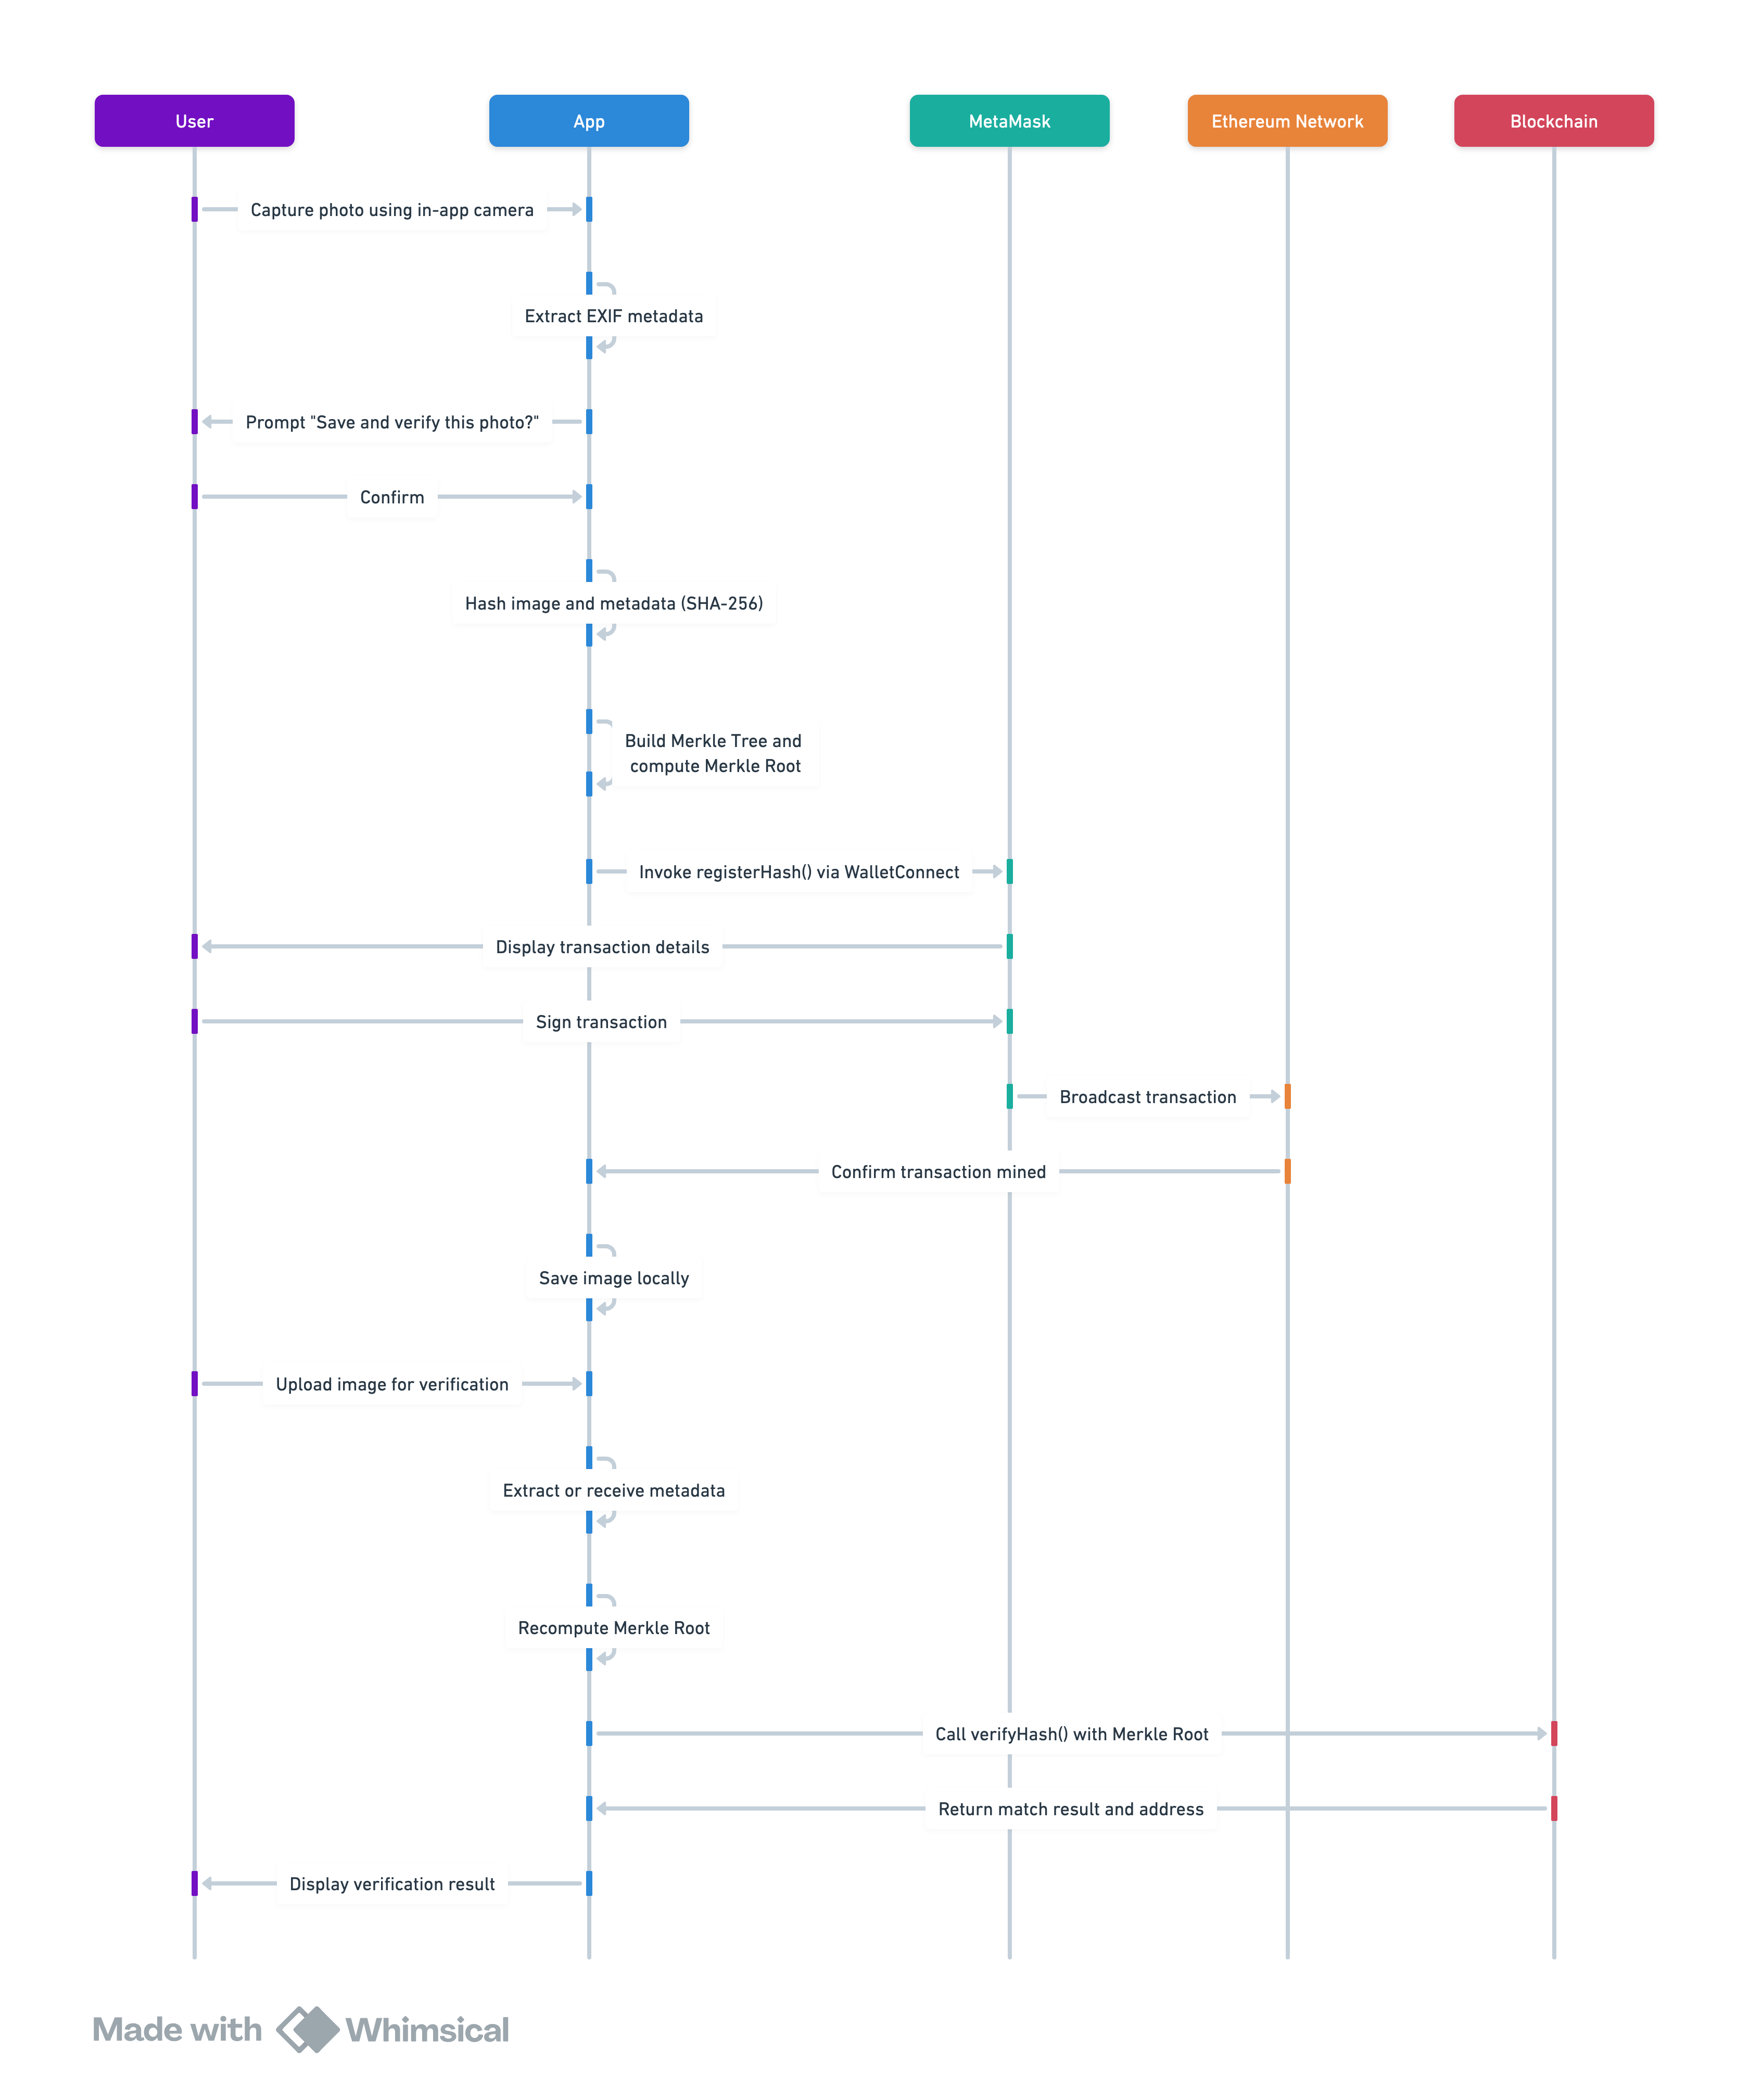
\includegraphics[width=0.90\textwidth]{images/sequenceDiagram.png}
    \caption{Sequence diagram: Capture and Verify}
    \label{fig:sequenceDiagramofCaptureAndVerify}
\end{figure}


\textbf{Instant Hashing and Registration}
A critical design goal of the proposed photo verification system is to eliminate the time window between image capture and verification, during which image manipulation or metadata tampering could occur. To address this, the system implements real-time hashing and on-chain registration immediately after a photo is captured. This design ensures that the image’s integrity is secured at the point of origin, making tampering infeasible without detection.

\subsection{Capture and Registration Flow}
This flow is triggered when a user captures an image using the in-app camera. The steps are:

\begin{figure}[htb]
    \centering
    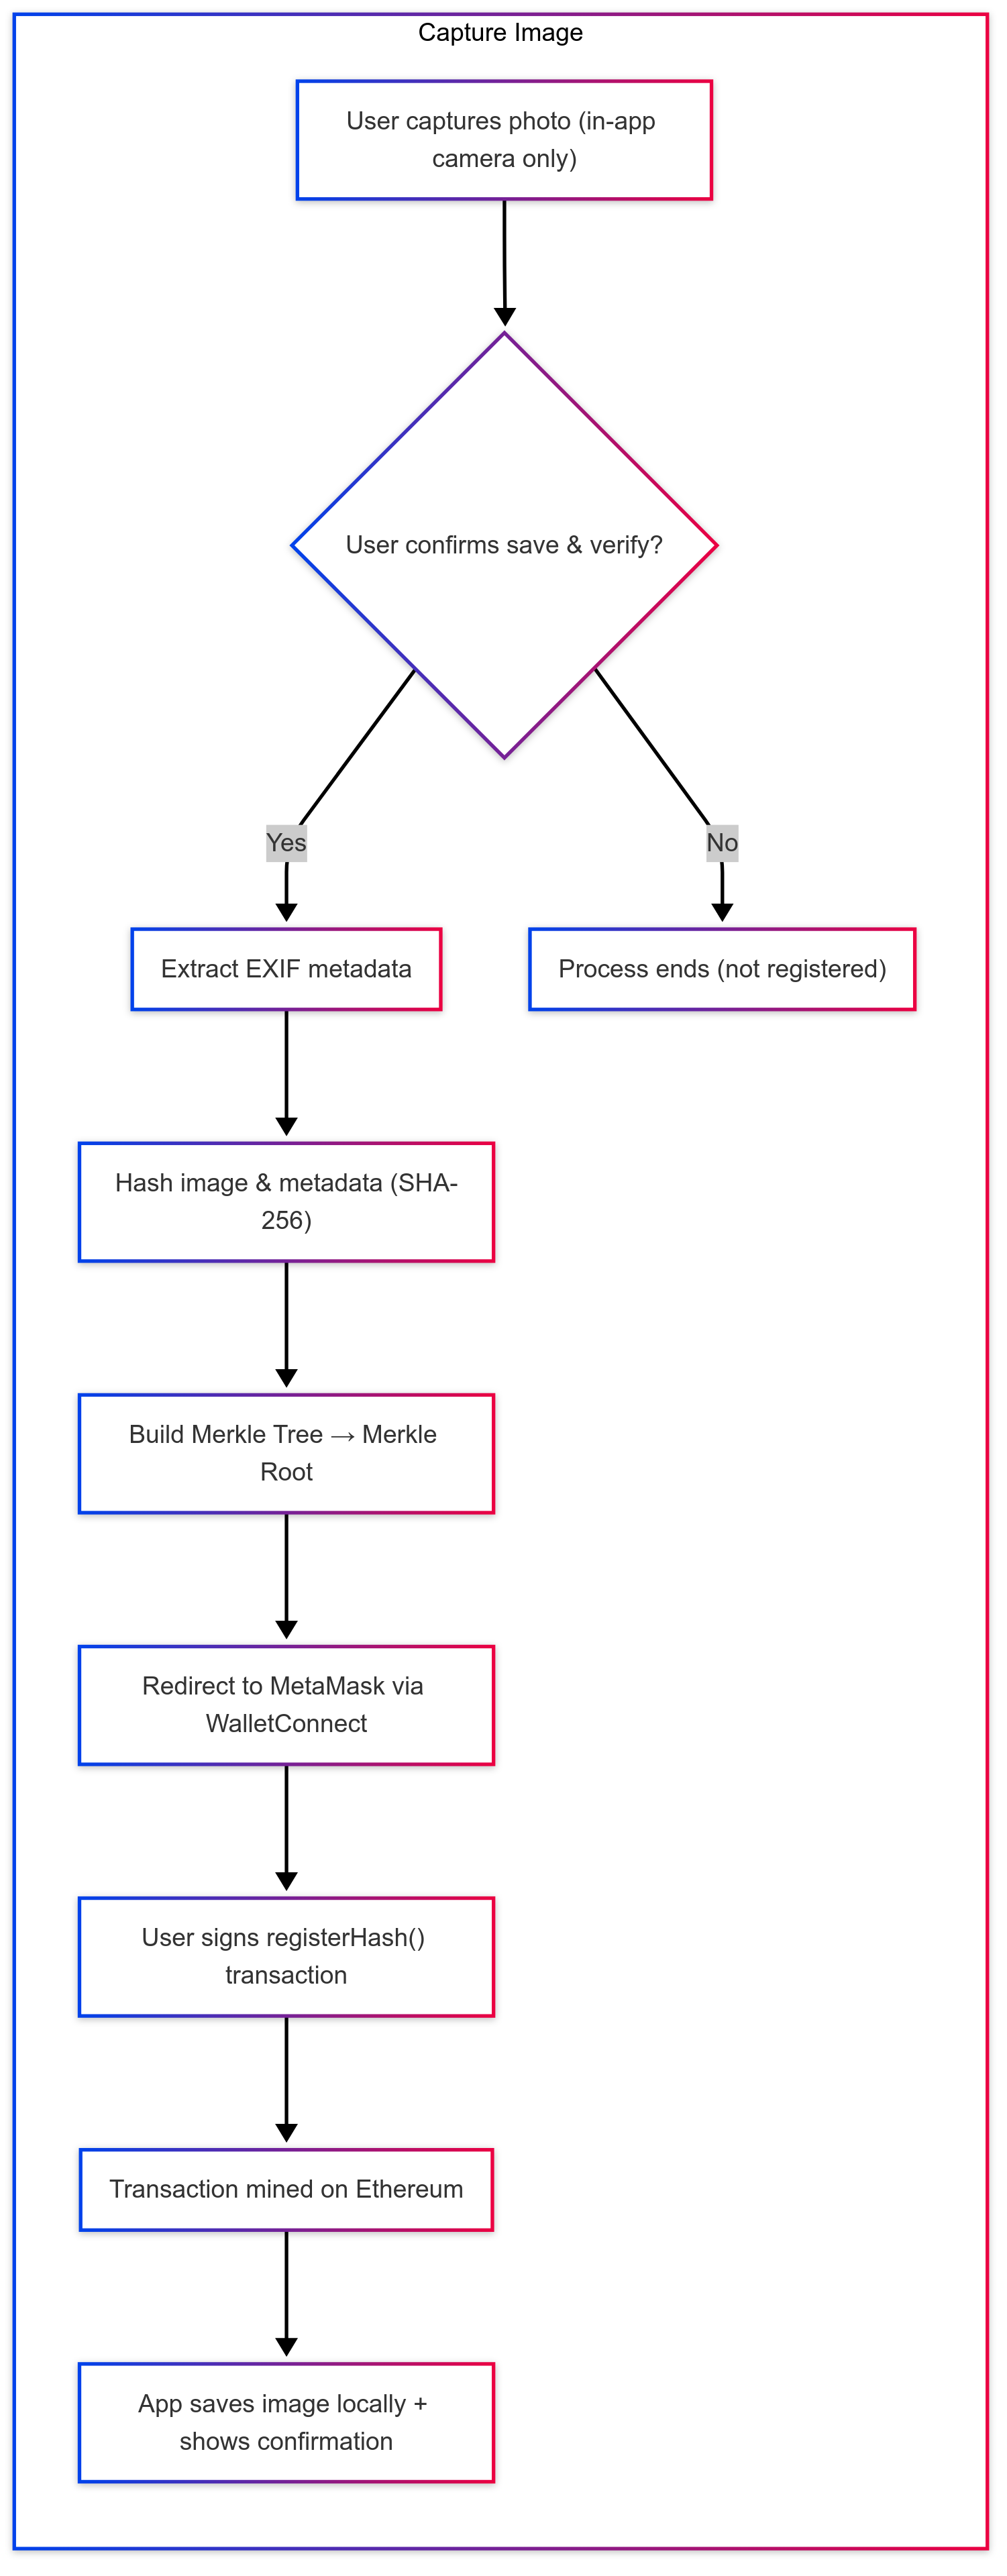
\includegraphics[width=0.50\textwidth]{images/captureImageFlow.png}
    \caption{Capture Image: Image Capture and Registration}
    \label{fig:imageCaptureAndRegistration}
\end{figure}

\begin{itemize}
    \item {\textbf{Image Capture:}} The user initiates photo capture through the app. This bypasses the system gallery or third-party apps to maintain control over the image lifecycle.
    
    \begin{figure}[H]
        \centering
        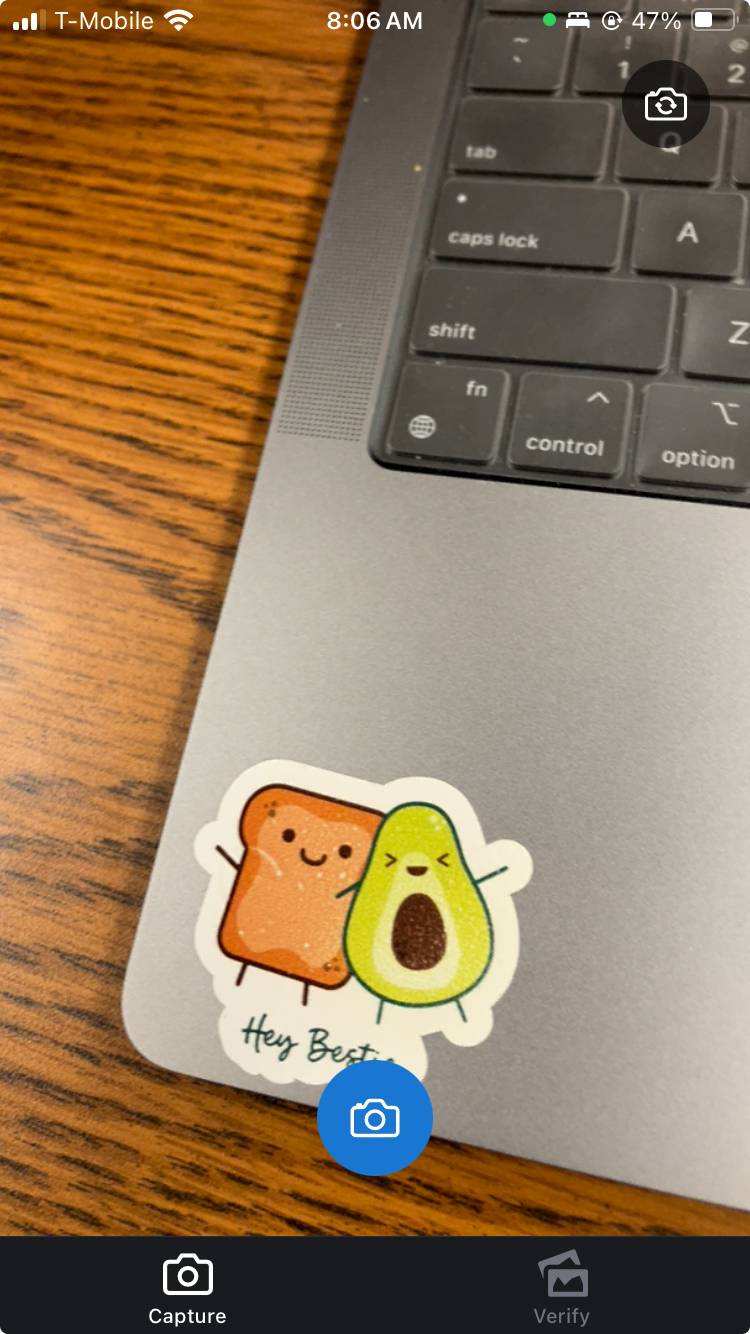
\includegraphics[width=0.30\textwidth]{images/imageCapture.jpeg}
        \caption{Capture Image: Image Capture UI}
        \label{fig:imageCapture}
    \end{figure}
    
    \item {\textbf{Confirmation Prompt:}} Immediately after capture, the app prompts the user to either:
    \begin{itemize}
        \item "Save and Register" (initiate verification and blockchain registration),
        \item Or "Discard" the image.
    \end{itemize}

    \begin{figure}[H]
        \centering
        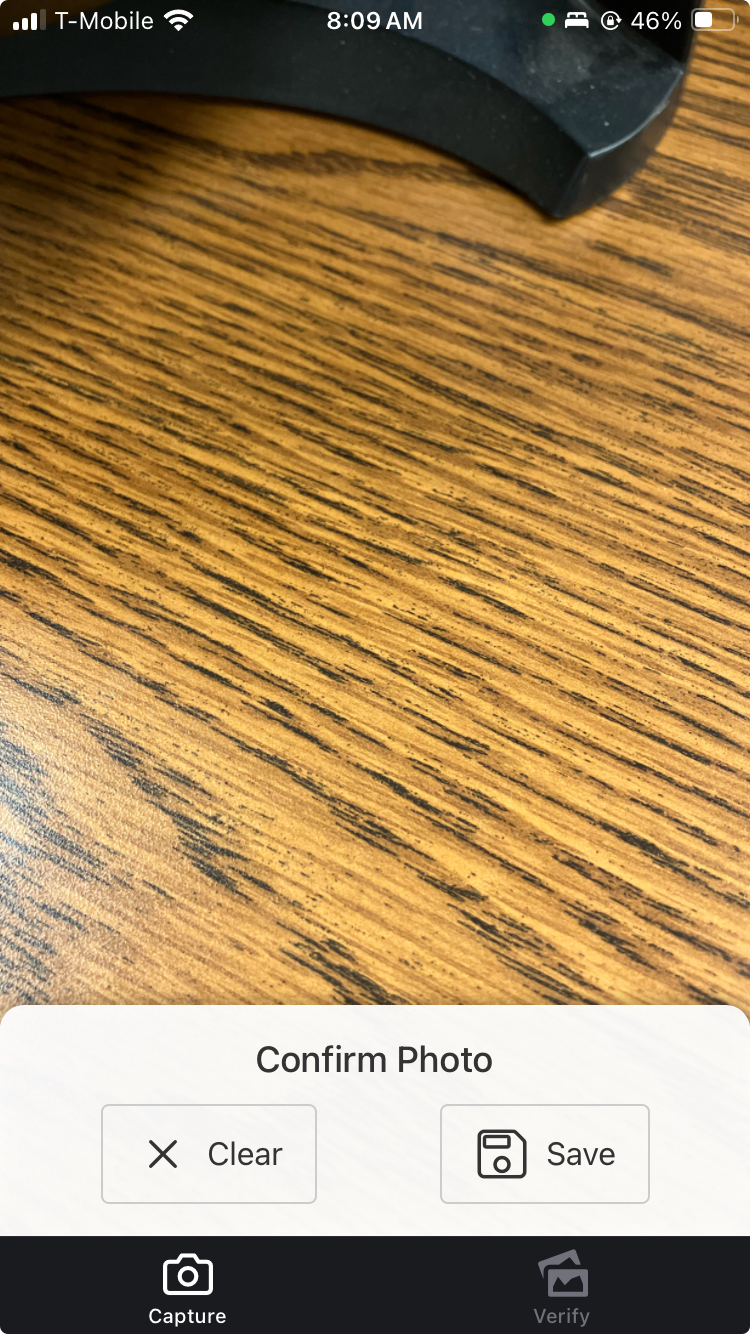
\includegraphics[width=0.30\textwidth]{images/confirmationPrompt.jpeg}
        \caption{Confirm Image: Image Confirmation Prompt}
        \label{fig:confirmationPrompt}
    \end{figure}

    \item {\textbf{Metadata Extraction:}} Upon confirmation, critical metadata is extracted from the image using iOS APIs. For any info that may not be available the value is defaulted to empty string(""). This capture metadata includes:
    \begin{itemize}
        \item Device and camera details (Make, Model, LensModel),
        \item Timestamps and GPS location,
        \item Resolution and exposure parameters.
    \end{itemize}

    \item {\textbf{Hashing and Merkle Root Computation:}} All metadata fields and the image content are hashed using SHA-256. These hashes are compiled into a Merkle Tree, and the resulting Merkle Root is computed.
    
    \item {\textbf{Blockchain Registration via MetaMask:}} 
    The application proceeds to call the registerHash() function of the smart contract after calculating the Merkle Root. 
    To maintain decentralization and ensure user control over their Ethereum identity, this transaction is not signed by the app itself. 
    The user is redirected to any of the 3rd party apps of their choice (e.g., MetaMask) to sign and confirm the transaction.
    \begin{itemize}
        \item The app passes the transaction data to MetaMask via deeplink or WalletConnect.
        \item The user reviews the transaction details, including gas fees and contract address in the specific app and then signs the transaction.
        \item Upon confirmation, MetaMask signs and broadcasts the transaction to the blockchain.
    \end{itemize}

    \begin{figure}[H]
        \centering
        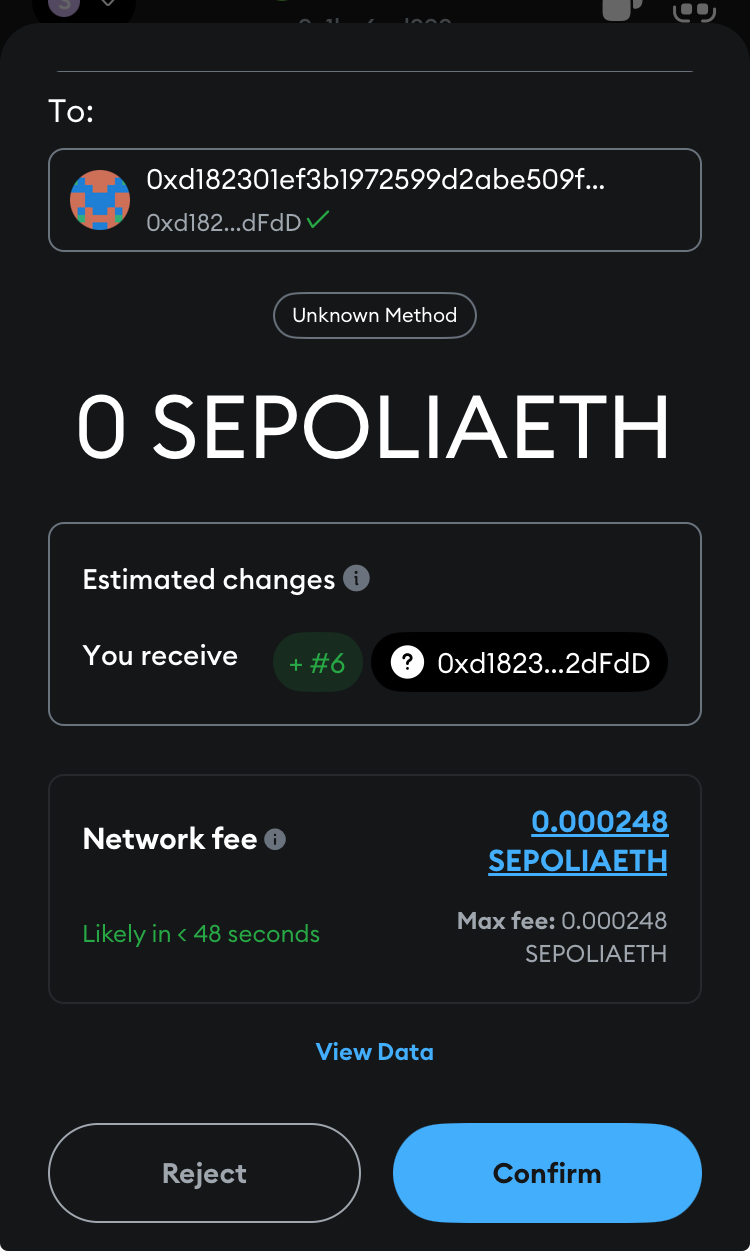
\includegraphics[width=0.30\textwidth]{images/blockchainConfirmation.jpeg}
        \caption{Blockchain Confirmation: Confirm Transaction on Metamask}
        \label{fig:blockchainConfirmation}
    \end{figure}

    \item {\textbf{Confirmation and Local Save:}} After the transaction is confirmed, the app receives a callback or event notification (e.g., via ethers.js or web3 polling) and proceeds to save the image locally. This finalizes the process. 
    \begin{figure}[H]
        \centering
        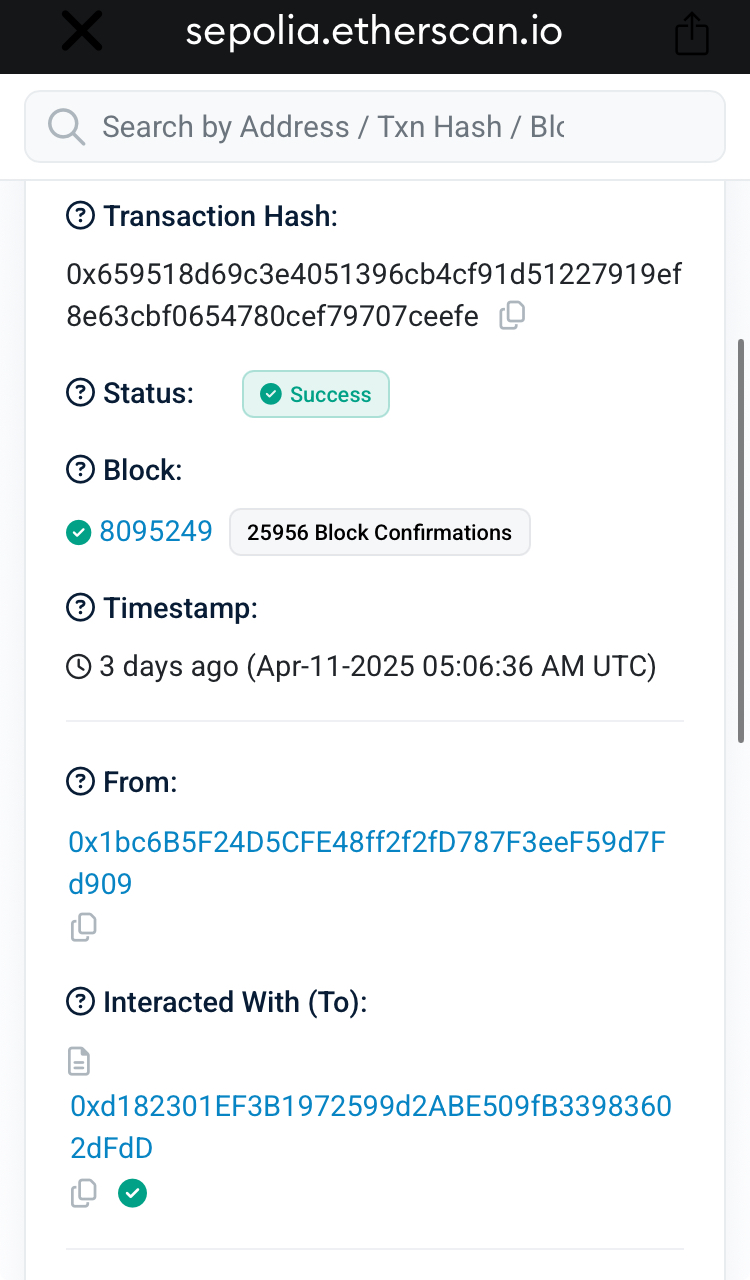
\includegraphics[width=0.30\textwidth]{images/etherTransactinConf1.jpeg}
        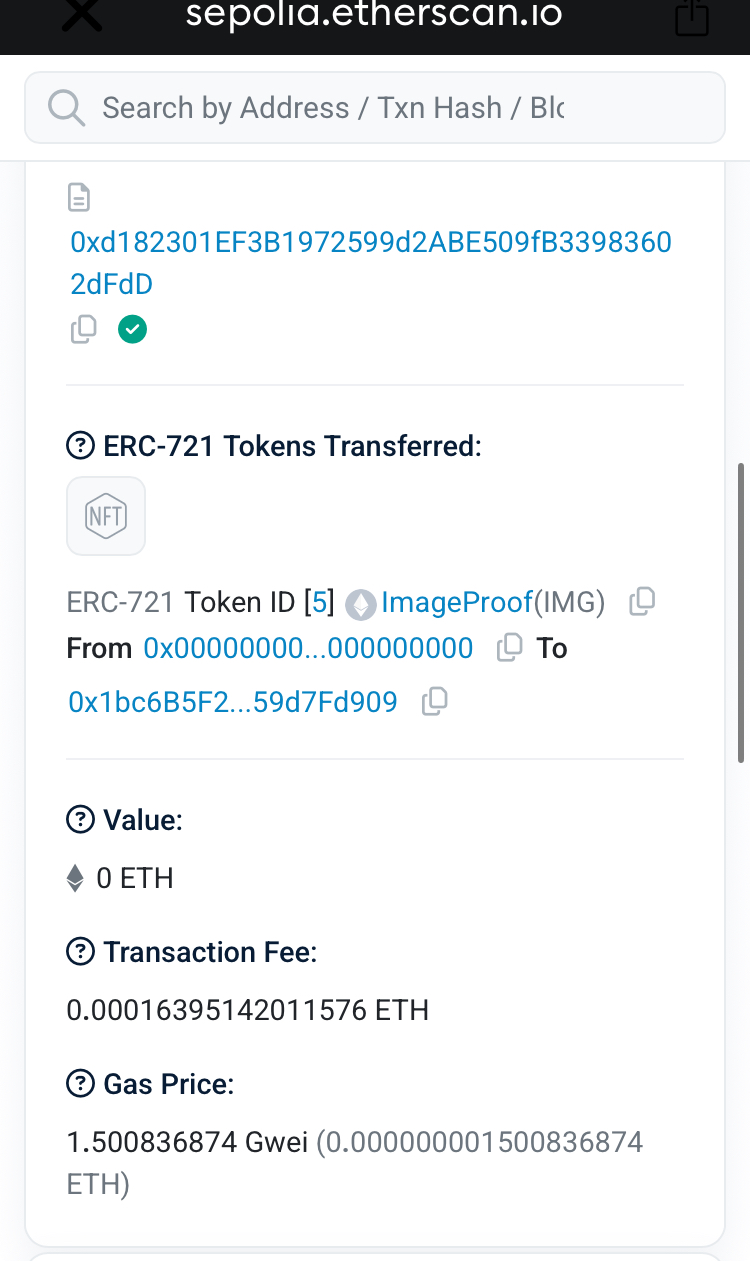
\includegraphics[width=0.30\textwidth]{images/etherTransactinConf2.jpeg}
        \caption{Blockchain Confirmation: Ethereum Testnet transaction confirmation}
        \label{fig:ethereuemConfirmation}
    \end{figure}
\end{itemize}

This flow ensures the image is cryptographically bound to its metadata and immutably registered on the blockchain at the point of capture leaving no opportunity for tampering between capture and storage.

\begin{figure}[ht!]
    \centering
    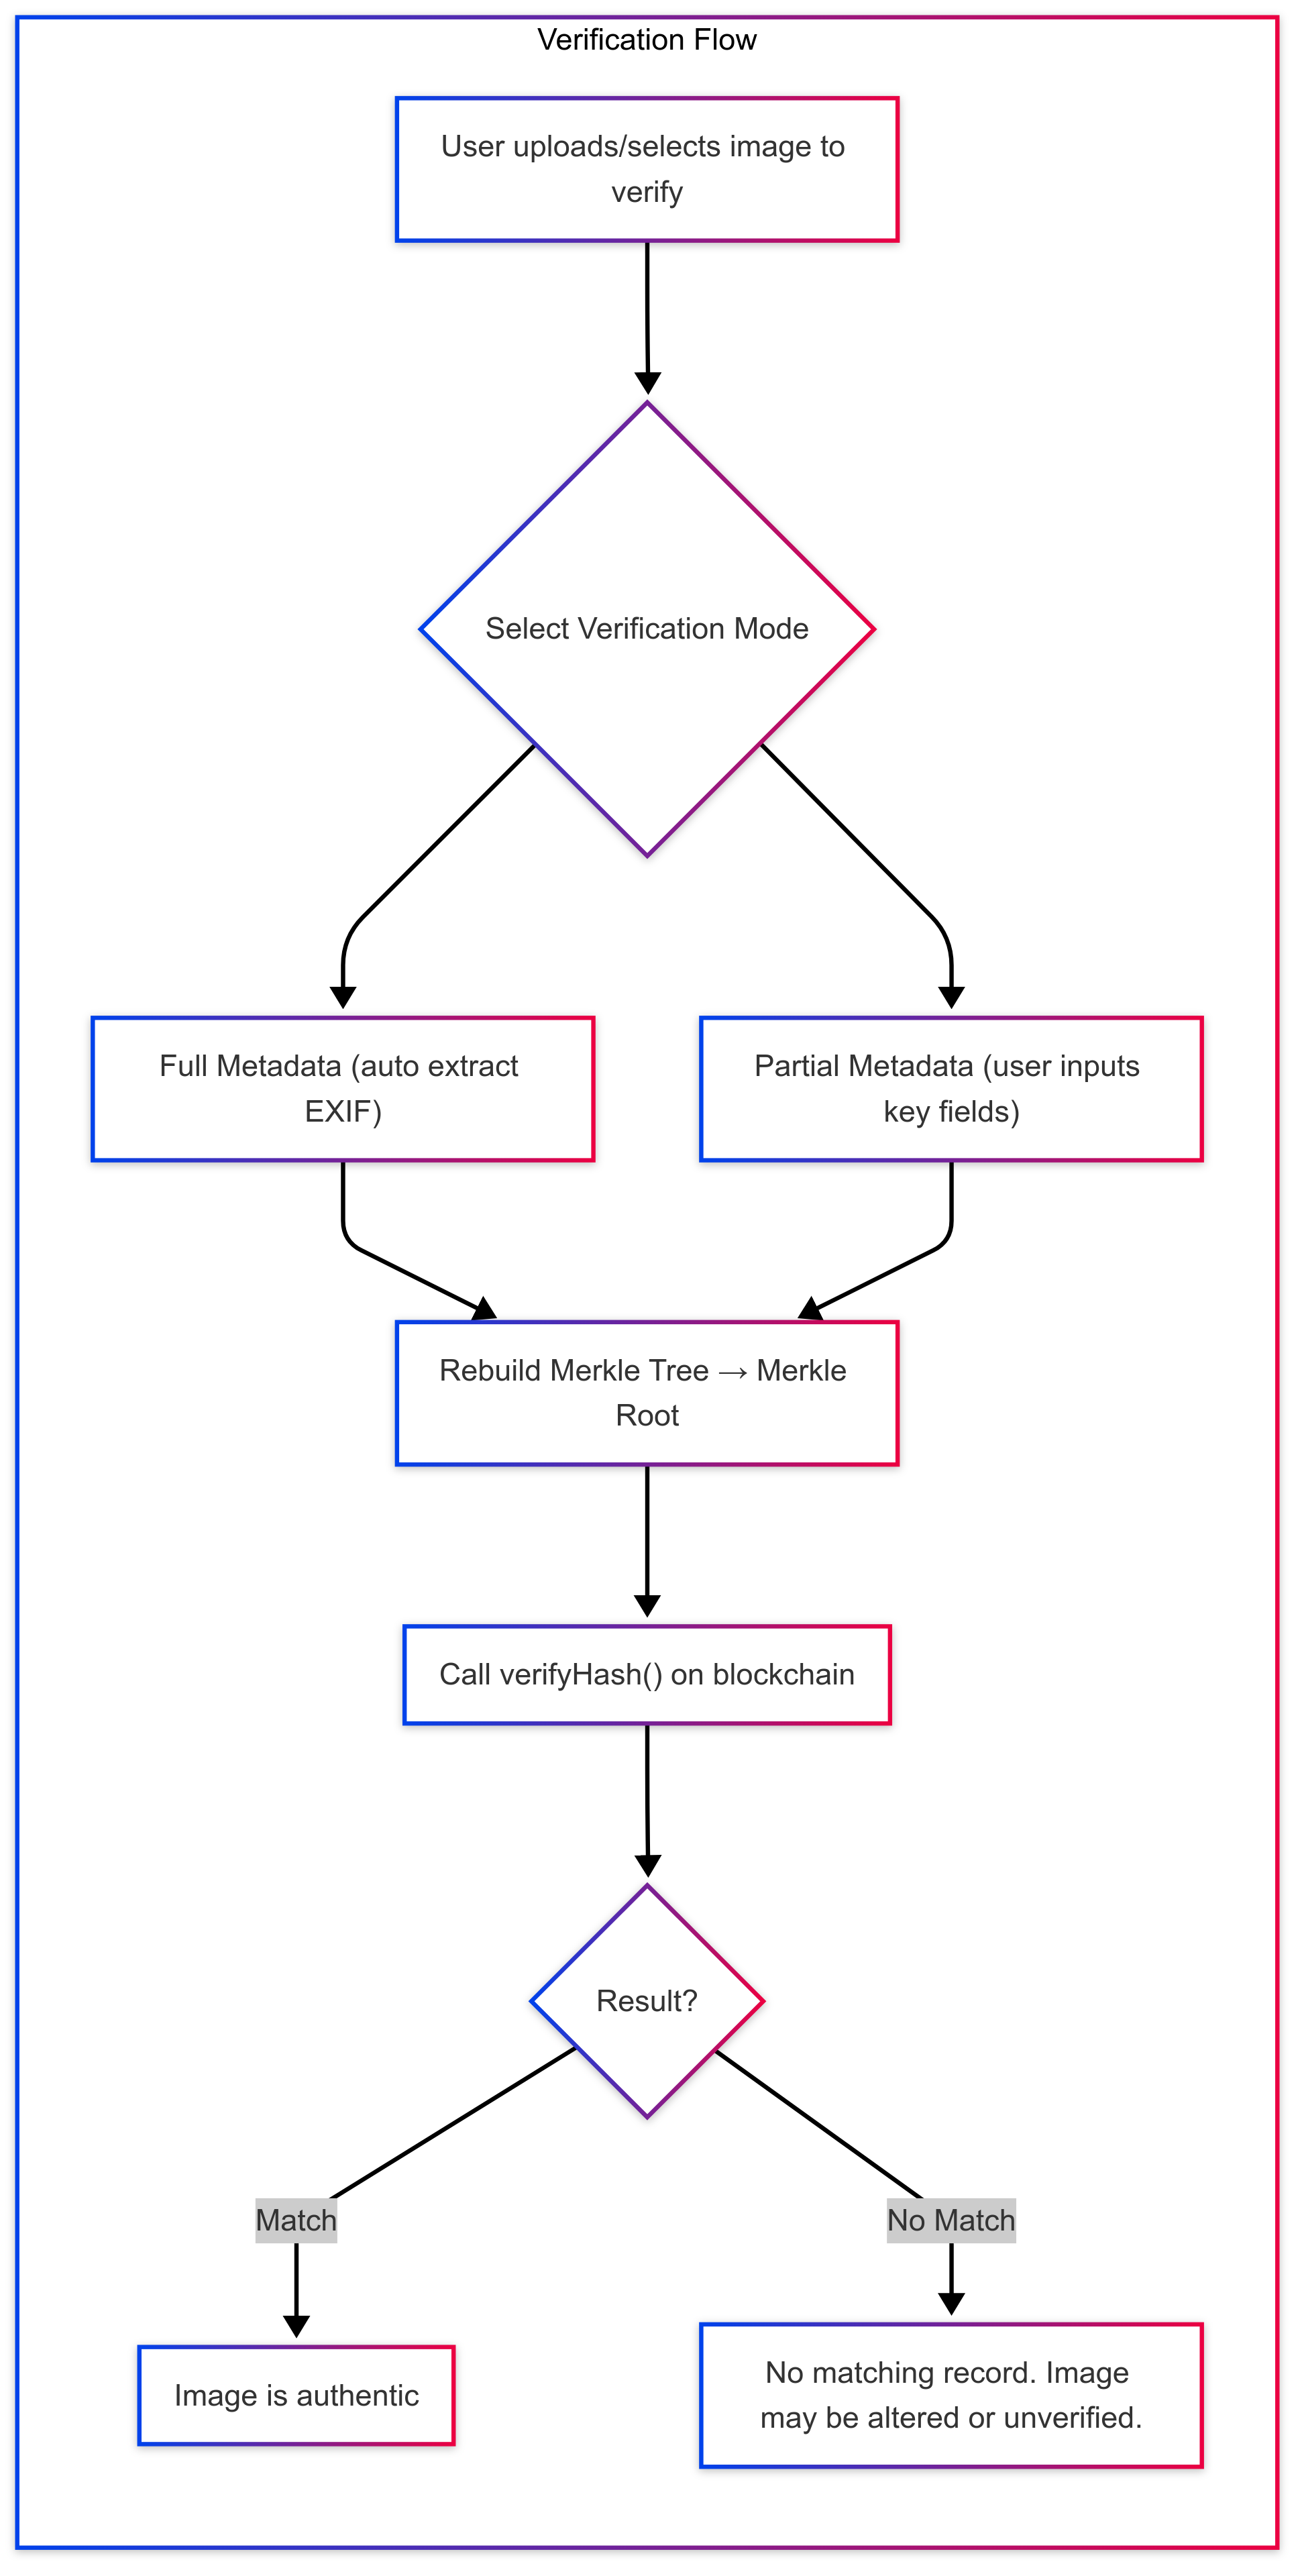
\includegraphics[width=0.65\textwidth]{images/verifyImageFlow.png}
    \caption{Verification Flow: Image Selection and Verification}
    \label{fig:verificationFlow}
\end{figure}

\subsection{Verification Flow}
This flow allows a user to validate whether a previously captured image is authentic. The steps are:
\begin{itemize}
    \item {\textbf{Verification Mode Selection:}} The app offers two modes:
    \begin{itemize}
        \item {\textbf{Full Metadata Verification:}} All metadata is extracted and included.
        \item {\textbf{Partial Metadata Verification:}} User manually enters critical fields (e.g., timestamp, device make) in case of missing metadata.
    \end{itemize}
        \begin{figure}[H]
            \centering
            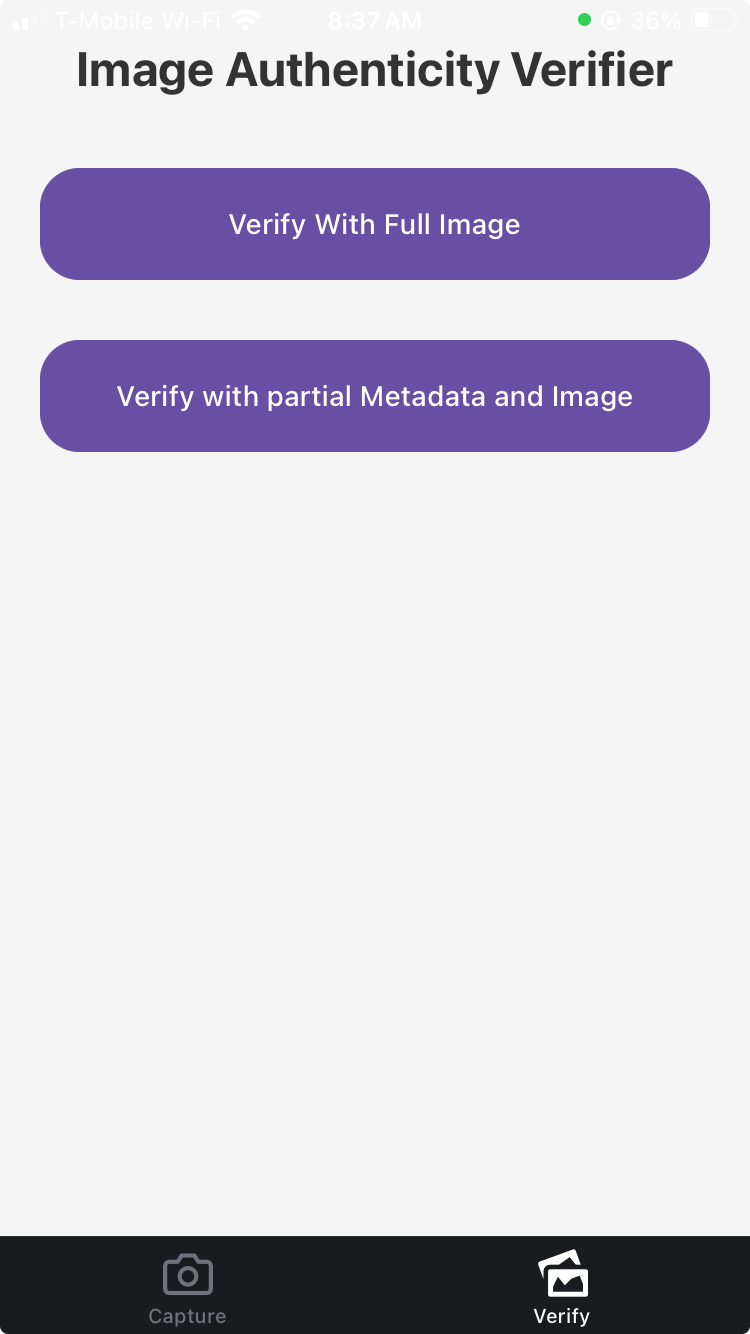
\includegraphics[width=0.30\textwidth]{images/verifyFlowRoot.jpeg}
            \caption{Verify Image: Choose flow}
            \label{fig:verificationRoot}
        \end{figure}

    \item {\textbf{Image Selection:}} The user selects an image from the app's gallery or camera roll.
        \begin{figure}[H]
            \centering
            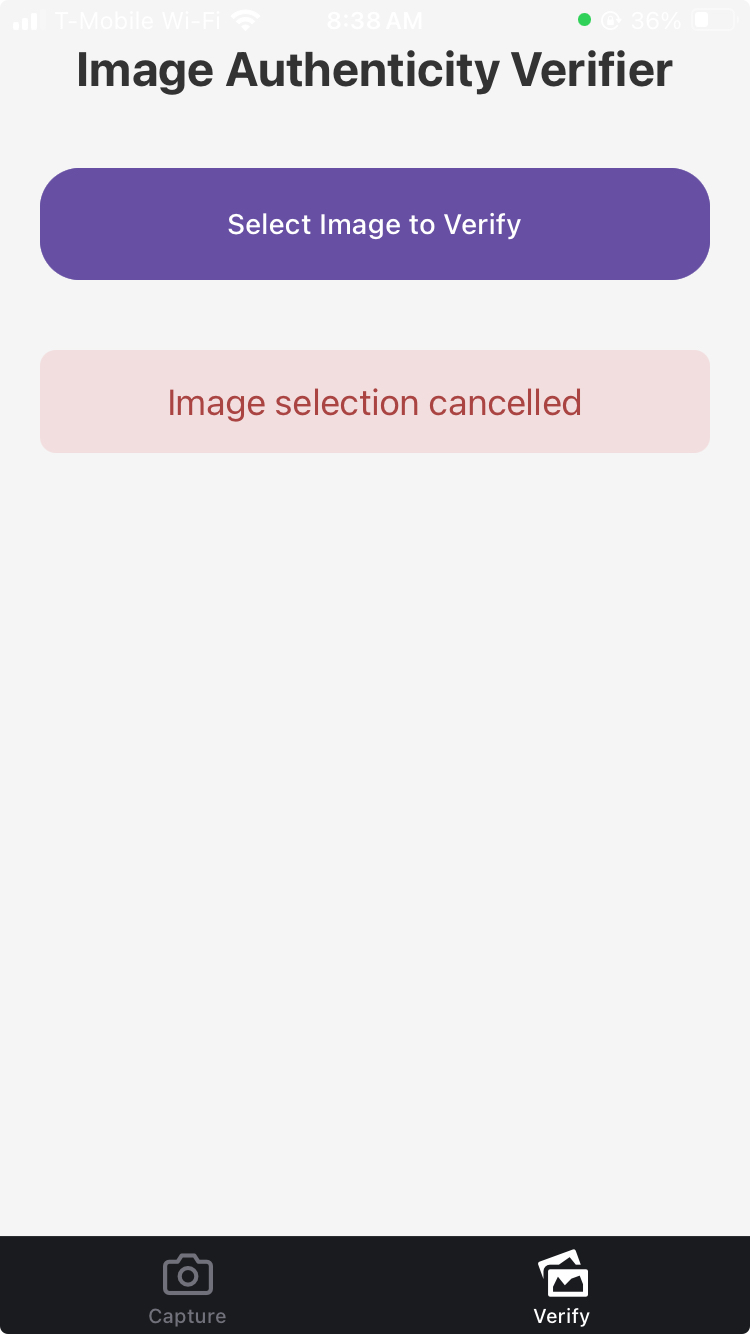
\includegraphics[width=0.30\textwidth]{images/selectImage.jpeg}
            \caption{Verify Image: Select Image}
            \label{fig:verifySelectImage}
        \end{figure}

    
    \item {\textbf{Recomputation of Merkle Root: }} The app re-hashes the image and selected metadata fields to reconstruct the Merkle Tree and compute the Merkle Root.
    \item {\textbf{Smart Contract Query:}} The Merkle Root is used to query the smart contract using the \textit{verifyHash()} function.
    \item {\textbf{Verification Result:}}
        \begin{itemize}
            \item If the hash exists on-chain, valid message is displayed.
            \item If the hash is not found, the app informs the user that the image is unverifiable.
        \end{itemize}
        \begin{figure}[H]
            \centering
            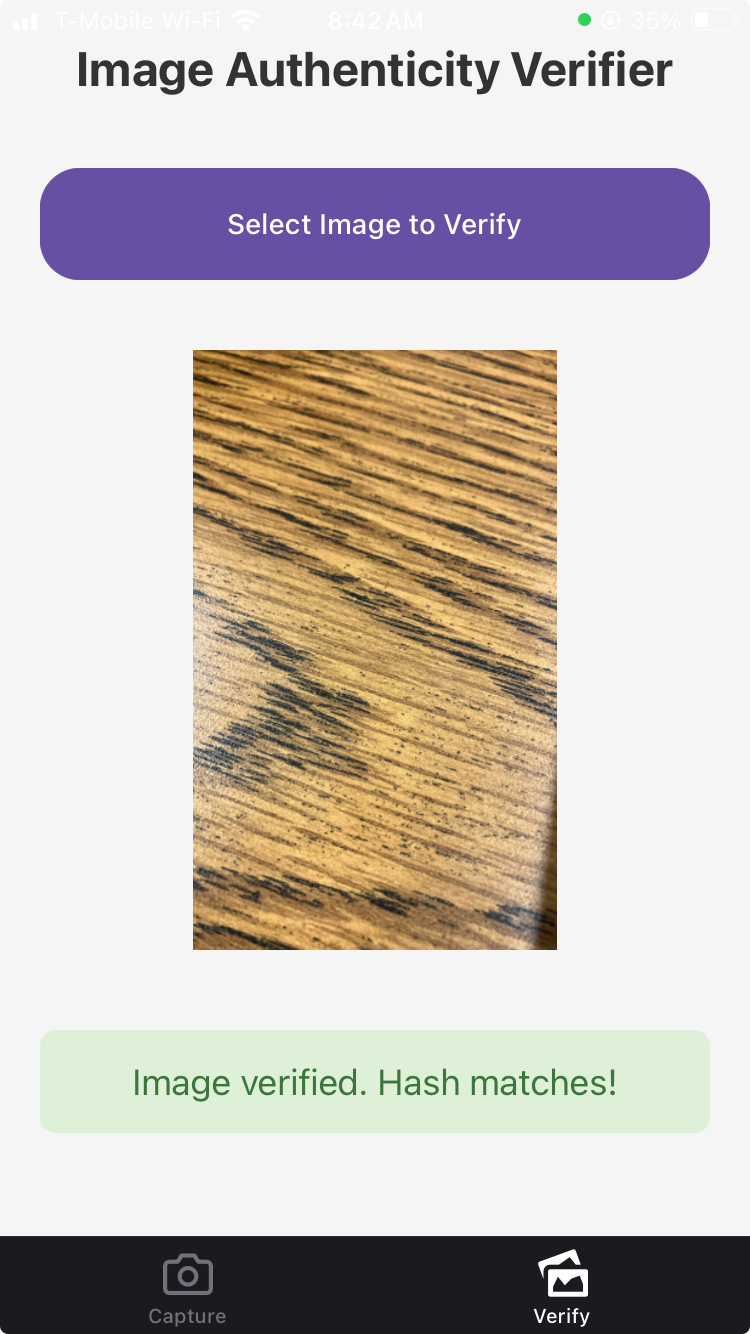
\includegraphics[width=0.30\textwidth]{images/verifySuccess.jpeg}
            \caption{Verify Image:  Successfully verified}
            \label{fig:verificationResultSuccess}
        \end{figure}

        \begin{figure}[H]
            \centering
            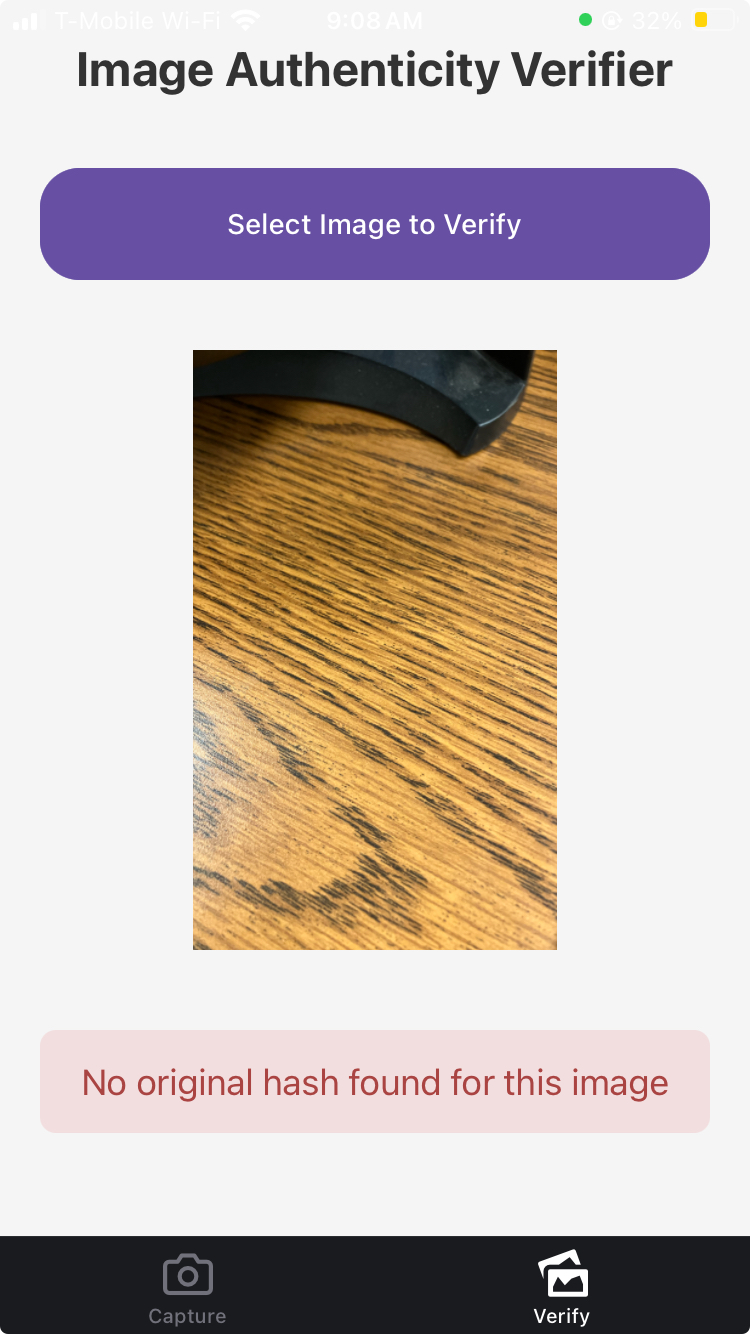
\includegraphics[width=0.30\textwidth]{images/verifyFailed.jpeg}
            \caption{Verify Image: Verification Failed}
            \label{fig:verificationResultFailed}
        \end{figure}
\end{itemize}


This verification process is instant due to the smart contract’s \textit{O(1)} lookup via \textit{mapping(bytes32 => address)}, and it incurs no gas fee as reads from the Ethereum blockchain are free.

\subsection{Design Considerations}
The UI is purposefully designed to be:

\begin{itemize}
    \item {\textbf{Minimalist}} – Clear, single-step prompts reduce cognitive load.
    \item {\textbf{Deterministic}} – Every action has one cryptographically verifiable outcome.
    \item {\textbf{Fail-Safe}} – Verification fails securely if metadata is missing or manipulated.
\end{itemize}

\subsubsection{Why 3rd Party Wallets?}
The decision to use 3rd party wallets like MetaMask for transaction signing is driven by several factors:
\begin{itemize}
    \item {\textbf{User Control:}} Users retain control over their private keys and transaction signing, reducing the risk of key exposure.
    \item {\textbf{Decentralization:}} The app does not hold or manage user funds, aligning with the principles of decentralization.
    \item {\textbf{Transparency:}} Users explicitly approve the registration transaction, reducing the risk of unauthorized actions.
    \item {\textbf{Security:}} 3rd party wallets are designed to handle sensitive operations securely, leveraging their established security protocols.
    \item {\textbf{Interoperability:}} Using widely adopted wallets ensures compatibility with various Ethereum networks and dApps.
\end{itemize}

The architecture design enables scalability through usability features which work alongside cryptographic requirements. The workflow follows trusted media standards \cite{harran2017} that require hashing to begin at acquisition time so each item develops an irreversible binding of its identity.


\section{Security and Code Integrity}
The digital media authentication process cannot be reduced to content protection alone because it demands a secure execution setting which safeguards both application logic and cryptographic operations and blockchain transactions from unauthorized changes. 
The system implements multi-layered security protocols which defend against tampering and spoofing and data leakage through mobile app and blockchain contract security measures.

\subsection{Mobile Application Security}
The application was developed exclusively for iOS because of its closed system and superior security features like application integrity guarantee and hardware-based key protection. 
The following technical features from iOS enable both runtime and distribution-level security:

\begin{itemize}
    \item {\textbf{Code Signing and App Store Validation: }} All application binaries require signature verification through Apple’s distribution certificates \cite{devCert}. 
    The signature process protects the application from modification or repackaging attempts because any unauthorized changes will invalidate the signature thus preventing reverse engineering and injection attacks \cite{iosSecGarg} \cite{benenson2013}.
    \item {\textbf{Sandboxing and App Isolation: }} Every iOS application operates within its own sandbox environment that blocks access to other applications' memory and data. The security mechanism blocks sensitive information from leaking while stopping unauthorized inter-process tampering \cite{iosSecGarg}.
    \item {\textbf{Secure Enclave and Keychain: }} Secure Enclave in iOS shields cryptographic operation processes such as key generation and digital signing of Ethereum transactions and hash verification by maintaining digital keys exclusively within secure hardware \cite{SecureEnclave2024}. The hardware-level guarantees power both metadata extraction and hashing processes \cite{benenson2013}.
    \item {\textbf{Runtime Integrity Checks: }} The application contains detection systems that identify standard runtime modifications including debugging and method swizzling and dynamic memory alterations to protect hash computation logic.
\end{itemize}

\subsection{Blockchain and Smart Contract Security}
The Solidity smart contract implements backend logic which operates from the Ethereum blockchain on the Sepolia Testnet Faucet. 
The system implements these design principles to establish trustlessness and prevent contract-level manipulation.

\begin{itemize}
    \item {\textbf{Minimal and Auditable Logic:}} The contract maintains a basic structure that focuses on a mapping(bytes32 => address) for image hashes to minimize potential vulnerabilities like reentrancy or overflow errors \cite{cheng2020}.
    \item {\textbf{Immutable Deployment:}} Once deployed, the contract cannot be altered/modified, and all interactions are logged immutably on the Ethereum ledger.
    \item {\textbf{Gas-Efficient Design:}} The transaction costs remain low with predictable execution times because all operations steer clear of unbounded loops together with dynamic storage arrays. The implementation follows optimization research recommendations to prevent denial-of-service attacks and excessive gas consumption \cite{chunmiao2021} \cite{Nguyen2022GasSaverAT}.
    \item {\textbf{Decentralized Identity Control:}} MetaMask transaction signing enables users to securely register hashes because it prevents unauthorized parties from making claims on their behalf.
\end{itemize}

\subsection{Obfuscation and Anti-Tampering Measures}
To protect the integrity of the hashing and metadata logic, the app uses industry-standard code obfuscation tools and best practices \cite{wandCodeObfuscation}. These include:

\begin{itemize}
    \item Renaming internal variables and function signatures.
    \item Removing unused code to minimize analysis surface.
    \item Implementing anti-debugging and anti-emulator detection routines at runtime .
\end{itemize}

These defensive measures create substantial expenses for reverse engineering while protecting against unauthorized modifications to hash generation or Merkle Tree building processes.


With hardware level security (Secure Enclave), software protections (code signing, sandboxing, obfuscation) and blockchain immutability, the system has a very high assurance environment that tightly controls the authenticity of the image and the behavior of the app. This holistic approach protects the data and the execution context, which is exactly what the project aims to achieve: trustworthy digital photo verification.